\documentclass{beamer}
\usepackage{graphicx}
\usetheme{Frankfurt}
\usecolortheme{beaver}

\title{Entity-based keyword search for web documents}
\author{Enrico Sartori}
\date{Academic Year 2010 - 2011}
\institute{University of Trento}

\begin{document}

\begin{frame}
\titlepage
\end{frame}

\section{Introduction}
\subsection{Current state}

\begin{frame}
\frametitle{Motivation}
Current search engines: {\bfseries Keyword based}\\
\bigskip
{\color{red}\bfseries{Advantages:}}\\
\bigskip
\begin{itemize}
\item Very popular in IR
\item Vector based similarity measures
\end{itemize}
\bigskip
{\color{red}\bfseries{Drawbacks:}}\\
\bigskip
\begin{itemize}
\item Ambiguity in natural language
\item Loss of information
\end{itemize}
\end{frame}

\subsection{Overview}

\begin{frame}
\frametitle{Overview}
Documents are {\bfseries complex objects:}
\bigskip
\begin{itemize}
\item Entities can be seen in the document
\item Relationships among entities described in documents
\item Documents are not just flat lists of words
\end{itemize}
\bigskip
Keyword-based approaches cannot catch these features of a document
\end{frame}

\subsection{Problem definition}

\begin{frame}
\frametitle{Problem definition}
User query as a flat list of keyword:
$$
q = \{kw_{1}, \dots, kw_{n}\}
$$
\begin{enumerate}
\item A document is relevant if it refers to the same \emph{entities}
  named in the query
\item Ranking of documents given by relationships matching
\end{enumerate}
\bigskip
\begin{exampleblock}{Entity}
Every real world object which can be uniquely identified
\end{exampleblock}
\end{frame}

\section{Solution}
\subsection{Document Representation}

\begin{frame}
\frametitle{Entities and relationships}
Entity-aware document model:
\begin{itemize}
\item Recognition of \emph{uniquely identified entities} inside the
  document
\item Document enriched with the entities identifiers
\end{itemize}
\bigskip
Relationships identification:
\begin{itemize}
\item Sentences summarization into triples
$$
t = (subject, verb, object)
$$
\item Verbs as actions involving entities
\item Each verb produces at least a triple
\end{itemize}
\bigskip
Document represented as the set of all the triples produced
\end{frame}

\subsection{Query Processing}

\begin{frame}
\frametitle{From a keyword query to a set of triples}
Translation of keyword query to a set of triples
\begin{itemize}
\item Entity recognition
\item Relationship identification
\end{itemize}
\vspace{5mm}
{\color{red}\bfseries{Algorithm overview:}}\\
\vspace{3mm}
\begin{tabular}{lcc}
User query as a set of keyword && $kw_{1}, kw_{2}, kw_{3}, kw_{4}$\\
& $\Downarrow$ &\\
Verbs and nouns recognition && $n_{1}, v_{1}, n_{2}, n_{3}$\\
& $\Downarrow$ &\\
Triples production && $(n_{1}, v_{1}, n_{2}), (n_{1}, v_{1}, n_{3})$\\
& $\Downarrow$ &\\
Entities recognition && $(e_{1}, v_{1}, n_{2}), (e_{1}, v_{1}, e_{2})$\\
\end{tabular}
\end{frame}

\subsection{Query Answering}

\begin{frame}{t}
\frametitle{Query Answering}
Similarity measure depends on relationships matching
\bigskip
\begin{columns}[T]
\column{.5\textwidth}
\begin{figure}
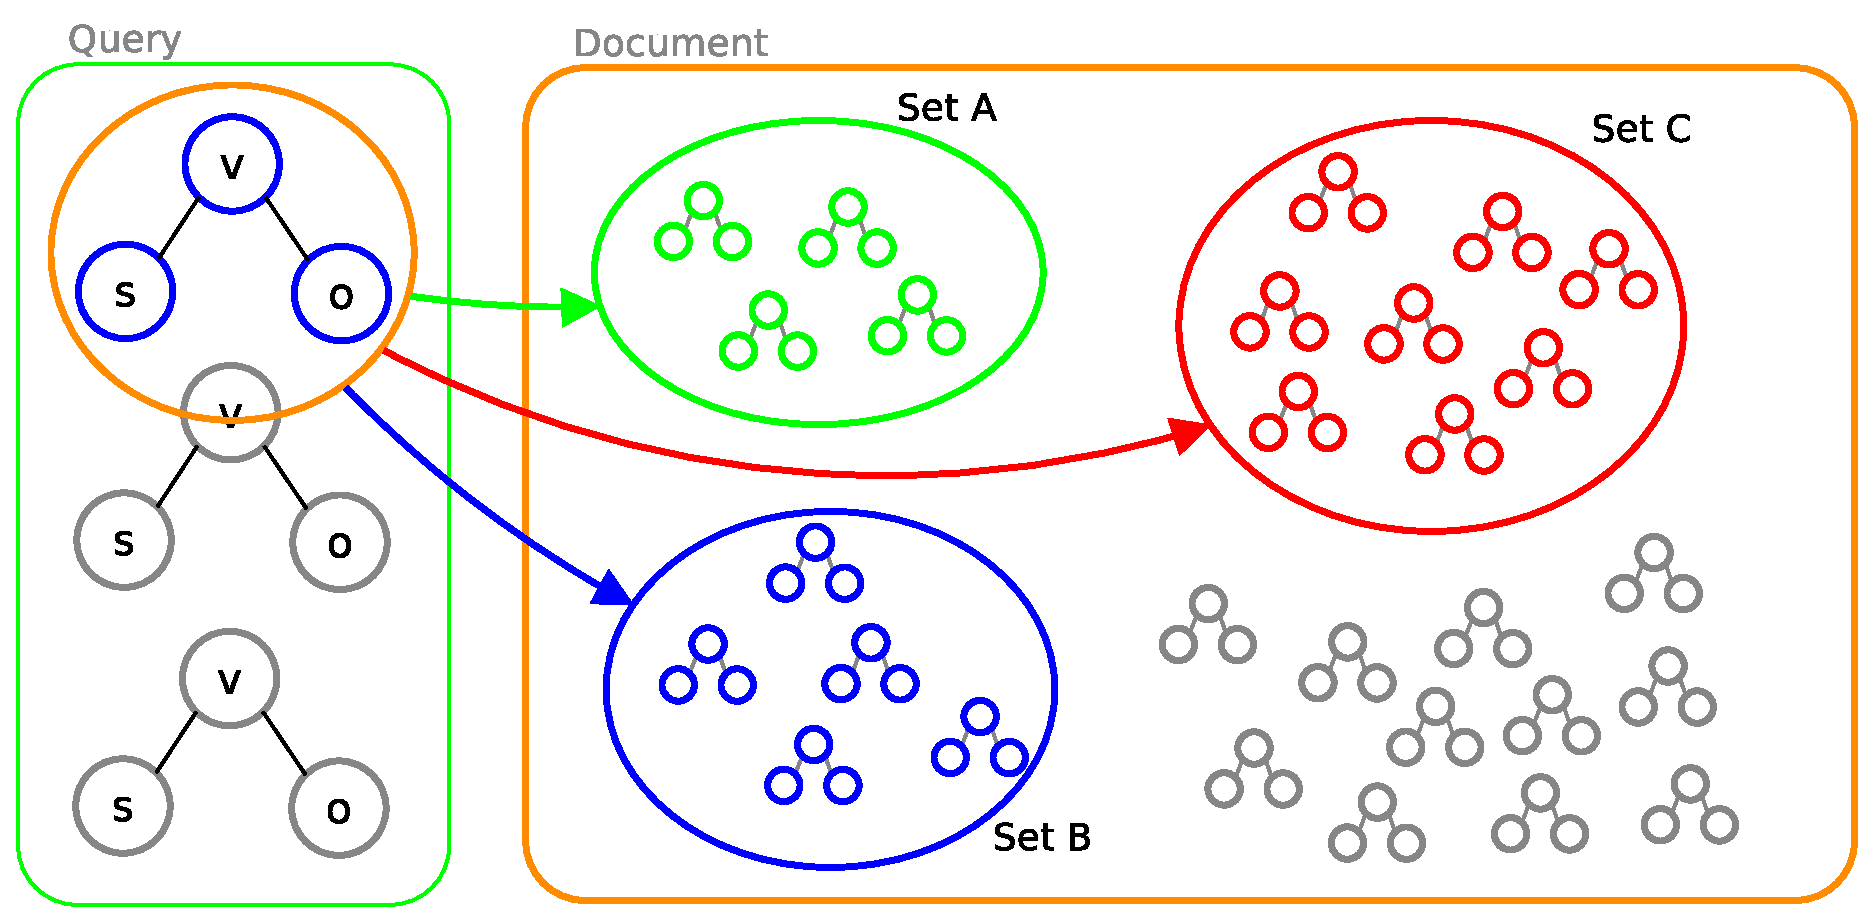
\includegraphics[scale=0.2]{imgs/sets}
\end{figure}
\column{.5\textwidth}
\begin{itemize}
\item {\bfseries{Set A:\\}} Totally matching triples
\item {\bfseries{Set B:\\}} Triples matching with \emph{subject} and \emph{object}
\item {\bfseries{Set C:\\}} Triples matching only with \emph{subject} or \emph{object}
\end{itemize}
\end{columns}
\bigskip
\vspace{1mm}
{\color{red}\bfseries{Similarity measure:}}
\tiny
$$
s_{1} = \frac{|\mathcal{A}|}{|\mathcal{D}|};\;
s_{2} = \frac{|\mathcal{B}|}{|\mathcal{D}| - |\mathcal{A}|};\;
s_{3} = \frac{|\mathcal{C}|}{|\mathcal{D}|-(|\mathcal{A}|+|\mathcal{B}|)}
$$
\small
$$
s (t, d) = s_{1} + (1 - s_{1}) \times
[s_{2} + (1 - s_{2}) \times s_{3}]
$$
\bigskip
\end{frame}

\subsection{Indexing}

\begin{frame}
\frametitle{Fast access to data}
Cardinality computation for sets A, B and C can be slow
\begin{itemize}
\item Indexing structure living in main memory
\item Index provides fast filtering of triples
\end{itemize}
\vspace{5mm}
The index should implement the following functions:\\
\vspace{2mm}
\begin{center}
\begin{tabular}{ll}
Set A: & $i_{\mathcal{A}} (s,v,o,d) = cnt_{s,v,o,d}$\\
Set B: & $i_{\mathcal{B}} (s,o,d) = cnt_{s,o,d}$\\
Set C: & $i_{\mathcal{C}} (s,o,d) = cnt_{s,d} + cnt_{o,d}$\\
\end{tabular}
\end{center}
\vspace{3mm}
Returns the number of triples satisfying the given parameters
\end{frame}

\section{Implementation}
\subsection{Entity recognition}

\begin{frame}
\frametitle{OpenCalais and Entity Recognition}
{\color{red}\bfseries{Document Pre-processing}}\\
Entities recognition system
\begin{itemize}
\item Integration of the OpenCalais REST webservice
\item High quality results and constant updates to data
\item Calling an external service presents latency issues
\end{itemize}
\bigskip
{\color{red}\bfseries{Query Answering}}\\
At query answering time no latencies acceptable
\begin{itemize}
\item Usage of local cache of OpenCalais data
\item Cache built at document pre-processing time
\end{itemize}
\end{frame}

\subsection{Relationships Identification}

\begin{frame}
\frametitle{Relationships Identification}
Identification of sentence grammatical structure
\begin{itemize}
\item Sentences and word tokenization
\item Part Of Speech tagging
\item Sentences grammar tree building
\item Summarization of grammar trees into triples
\end{itemize}
\bigskip
{\color{red}\bfseries{Query Answering}}\\
Simpler and time-saving approach
\begin{itemize}
\item Queries don't follow natural language grammar rules
\item Ordering of keywords important to recognize relationships
\end{itemize}
\end{frame}

\subsection{Indexing}

\begin{frame}
\frametitle{Index implementation}
The index structure is an adaptation of the Hexastore approach
\begin{columns}
\column{.4\textwidth}
\begin{figure}
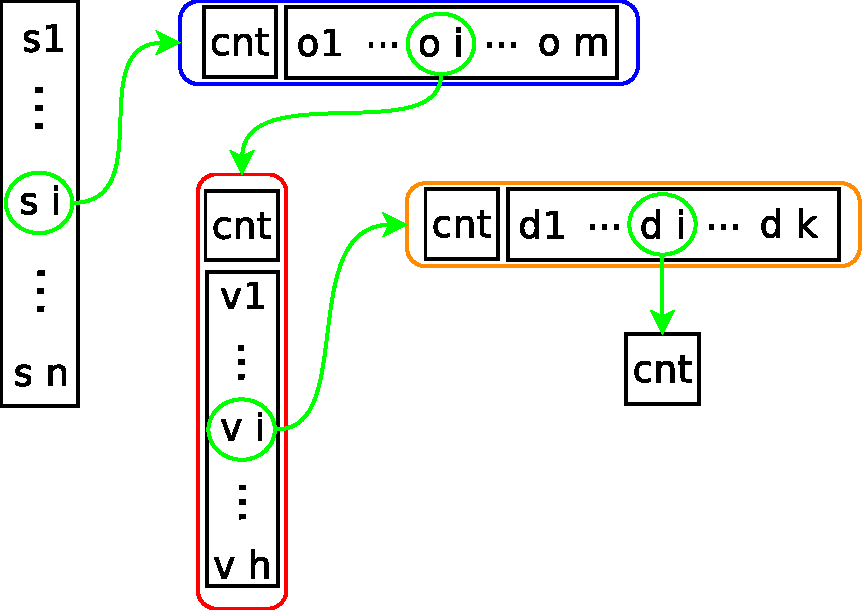
\includegraphics[scale=0.35]{imgs/index}
\end{figure}
\column{.6\textwidth}
\begin{itemize}
\item Nested associative arrays
\item Values of the triples fields as keys
\item Index counts the triples matching the given parameters
\end{itemize}
\end{columns}
\bigskip
Different arrangements of the arrays can compute the cardinality of the
three subsets
\end{frame}

\section{Experiments}
\subsection{Document preprocessing}

\begin{frame}
\frametitle{Document preprocessing time}
\begin{figure}
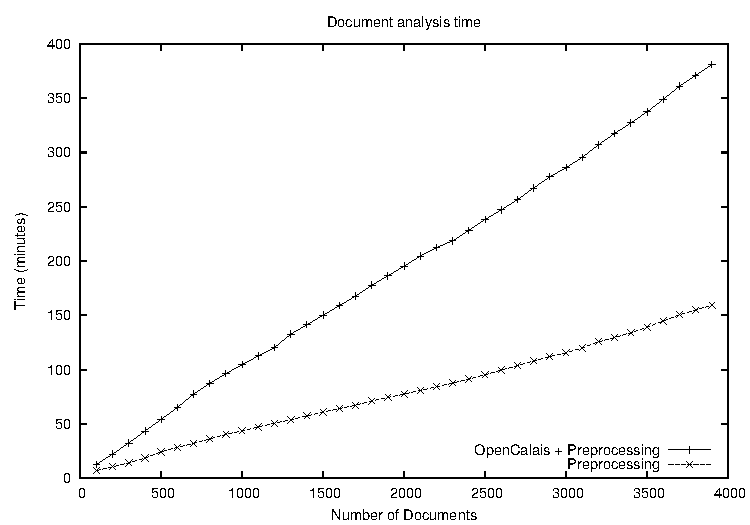
\includegraphics[scale=0.6]{imgs/analysis_time}
\end{figure}
\begin{columns}[T]
\column{.5\textwidth}
\centering
\tiny
\begin{tabular}{l|c}
TASK & TIME \\
\hline
\bf{Query OpenCalais:} & \bf{3.375 s}\\
\;\;Read file: & 0.001 s\\
\;\;Query service: & 3.359 s\\
\;\;Storage time: & 0.014 s\\
\end{tabular}
\column{.5\textwidth}
\centering
\tiny
\begin{tabular}{l|c}
TASK & TIME \\
\hline
\bf{Analysis time:} & \bf{1.917 s}\\
\;\;Read file: & 0.015 s\\
\;\;Entities marking: & 0.004 s\\
\;\;Sentences analysis: & 1.797 s\\
\;\;DB storage: & 0.775 s\\
\end{tabular}
\end{columns}
\bigskip
\end{frame}

\subsection{Query answering}

\begin{frame}
\frametitle{Query processing and answering}
\begin{columns}[T]
\column{.5\textwidth}
\centering
\begin{figure}
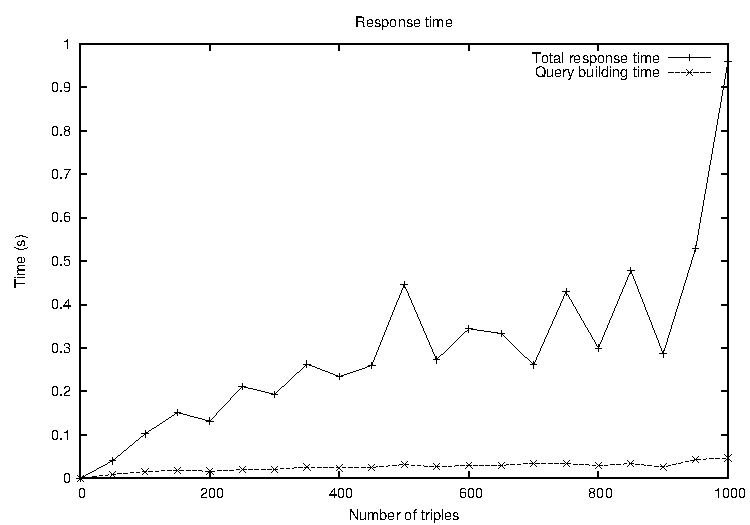
\includegraphics[scale=0.46]{imgs/qr_time_tot}
\end{figure}
\column{.5\textwidth}
\centering
\begin{figure}
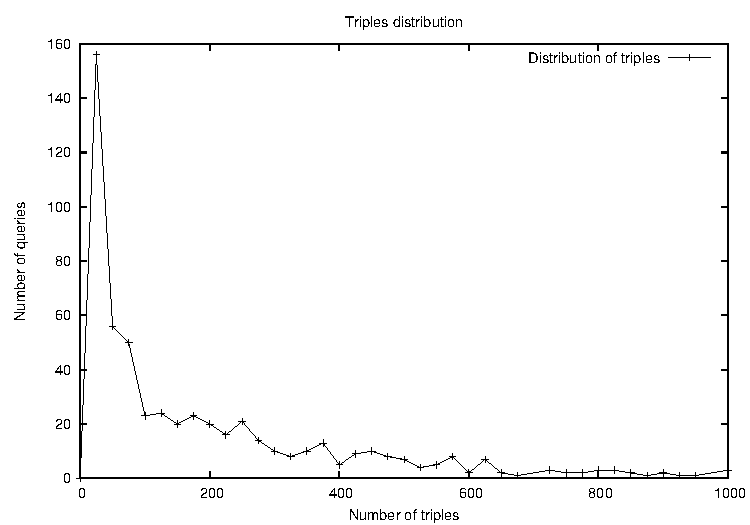
\includegraphics[scale=0.46]{imgs/qr_tris_tot}
\end{figure}
\end{columns}
\bigskip
Most of the user queries produce less than 400 triples, and the system
responds to them in less than 0.3 s\\
\bigskip
Fluctuation in the plot are caused by different values present in the
triples
\begin{itemize}
\item Wildcard values reduce the number of lookups in the index
\end{itemize}
\bigskip
\end{frame}

\subsection{Indexing}

\begin{frame}
\frametitle{Indexing time and memory usage}
\begin{columns}[T]
\column{.5\textwidth}
\centering
\begin{figure}
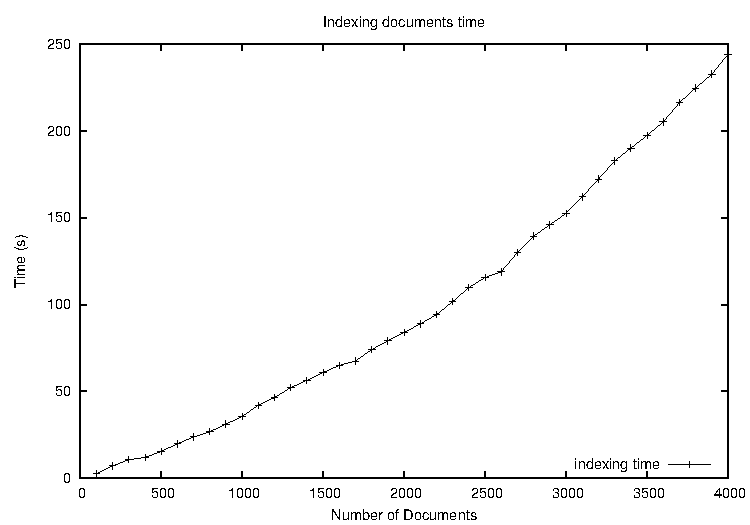
\includegraphics[scale=0.46]{imgs/index_time_d}
\end{figure}
\column{.5\textwidth}
\centering
\begin{figure}
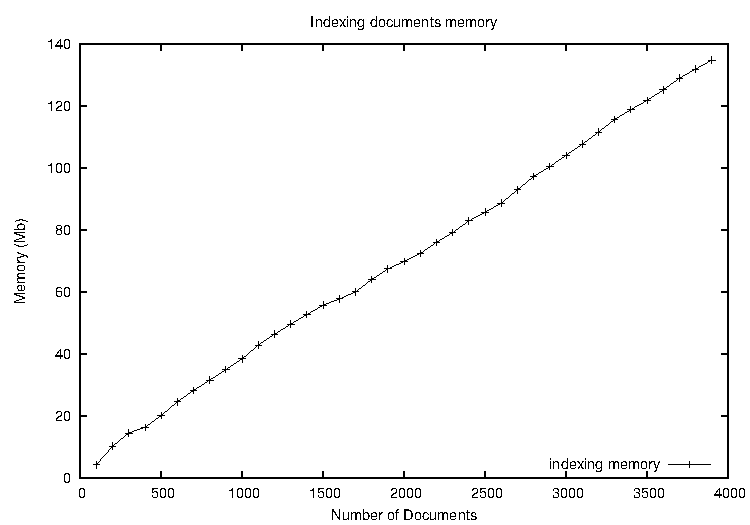
\includegraphics[scale=0.46]{imgs/index_memo_d}
\end{figure}
\end{columns}
\bigskip
Time needed to build the index and memory usage grow almost linearly
with the number of documents.\\
\bigskip
\begin{itemize}
\item Index structure built at startup
\item Supports incremental updates as new documents appear
\end{itemize}
\bigskip
\end{frame}


\section{Conclusions}
\subsection{Conclusions}

\begin{frame}
\frametitle{Conclusions and future work}
\begin{itemize}
\item Definition of a novel approach to document representation and
  query answering
\item Document model entity-based and defined in terms of
  relationships among objects
\item Document similarity computation based on relationships matching
\end{itemize}
\bigskip
{\color{red}\bfseries{Further developments and possible improvements}}\\
\begin{itemize}
\item Improvement of presented algorithms for relationships
  identification
\item Limit the number of triples produced in query answering
\item Adapt the approach to different setting of application
\end{itemize}
\end{frame}

\section*{}
\begin{frame}
\begin{center}
\begin{figure}
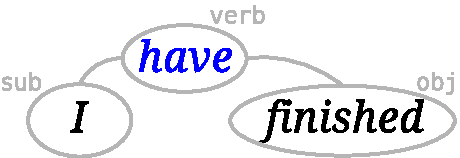
\includegraphics[scale=0.6]{imgs/joke}
\end{figure}
\bigskip
Thank you for your attention!\\
Questions?
\end{center}
\end{frame}

\end{document}
